\documentclass{article}
\usepackage{graphicx}


\setlength{\parskip}{1em}

\begin{document}


\title{Resource Components}

Resource Components are ICE Components which contain a grid of visualization resources. These resources can display files from a variety of sources, such as CSV files or VisIt visualizations.

\section{Prerequisites}

This tutorial assumes that the class you are writing already has an ICE Form. If you are writing an extension of ICE's Item class, then the work of creating and managing a Form is already done for you. You can still give the item your own Form using the submitForm function.

If you are writing your own class, simply instantiate Form or any of its
subclasses.

\section{Adding the Component}

First, create a new resource component.

\begin{verbatim}
ResourceComponent resourceComponent = new ResourceComponent();
\end{verbatim}

Set the component's name, description, and ID.

\begin{verbatim}
resourceComponent.setName("Resources");
resourceComponent.setDescription("Results");
resourceComponent.setId(2);
\end{verbatim}

Add the component to your class's form.

\begin{verbatim}
form.addComponent(resourceComponent);
\end{verbatim}

\section{Adding Resources to the Component}

Now that the component is ready, you can add Resources to it. Begin by
initializing the resource.

\begin{verbatim}
VizResource visResource = new VizResource(file);
\end{verbatim}

The file in the above code should be an IFile pointing to the file you
wish to display, such as an output file written by some other part of your
class. If you are extending an Item, you can simply get the file from the
project.

\begin{verbatim}
VizResource visResource = 
	new VizResource(project.getFile("Filename");
\end{verbatim}

Otherwise, you will need to create your own IFile instance.

As an example, add the following two resources to the component.

\begin{verbatim}
VizResource csvResource = new 
	VizResource(project.getFile("fib8.csv");
VizResource visItResource = new 
	VizResource(project.getFile("wave.visit");
\end{verbatim}

This will add a graph and a VisIt plot to your resources component. After
creation, you can now add the resources to the component.

\begin{verbatim}
resourceComponent.add(csvResource);
resourceComponent.add(visItResource);
\end{verbatim} 

\section{Using the Resource Component}

\subsection{Establishing a VisIt Connection}

In order to visualize resources containing VisIt files, ICE must be connected to
a running VisIt installation. To set up this connection, select Windows
$\rightarrow$ Preferences... in ICE's menu bar. (On Mac OS X, Preferences is
instead located under Eclipse ICE in the menu bar.)

\begin{center}
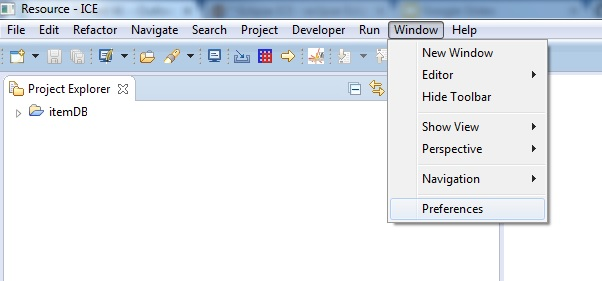
\includegraphics[width=12cm]{images/ICEPreferences}
\end{center}

Select Visualization $\rightarrow$ VisIt in the tree on the left side of the
Preferences window.

\begin{center}
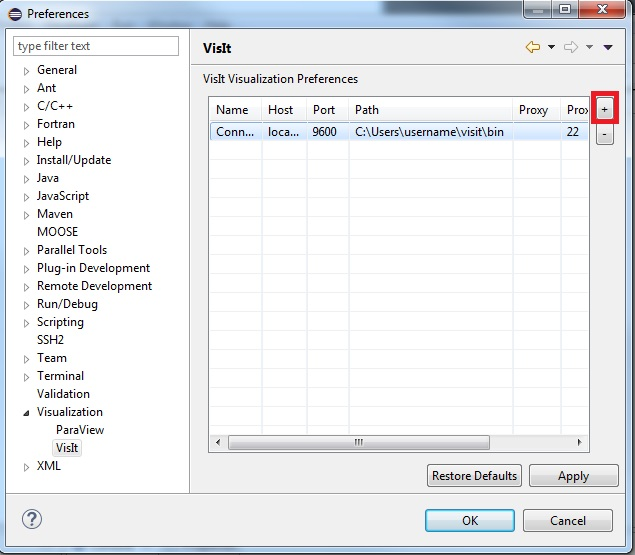
\includegraphics[width=12cm]{images/VisualizationPreferences}
\end{center}

Press the button with a "+" symbol in the upper right (highlighted in the image
above) to add a new row to the table. Click on the Path cell of the new row and
put the path of your installation of VisIt.

Press Apply, then OK, both in the lower right hand corner. ICE will now open and
connect to this VisIt installation each time ICE is opened.

\subsection{Managing the Resources}

Once you open your Item in ICE, you should notice a new tab inside containing
your ResourceComponent. Its title will be whatever you set as its description
when creating the code for it.

At the top left of the screen will be controls for the component's layout.

\begin{center}
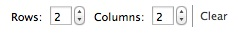
\includegraphics{images/ResourceComponentControls}
\end{center}

The Clear button will close all plots in the component. The other two controls
will allow you to specify the number of rows and columns in the grid. Be careful
when reducing them, as any plots which no longer fit in the grid will be closed.

If you hover over a plot, a button will appear in the upper left hand corner.
Clicking it will close that plot. 

\begin{center}
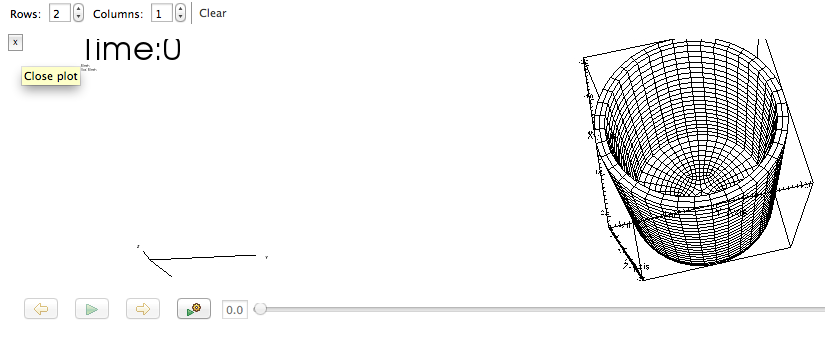
\includegraphics[width=12cm]{images/ClosePlotButton}
\end{center}

\subsection{Interacting with CSV Plots}

The top of the CSV plot has a row of buttons which control various aspects of
the graph's presentation.  

\begin{center}
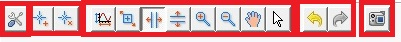
\includegraphics[width=12cm]{images/CSVControls}
\end{center}

From left to right, the buttons are:

1) Control basic parts of the graph, such as the font, axis titles and scales,
line colors, etc.

2-3) Add or remove, respectively, annotations for specific data points.

4-11) These buttons contain a variety of different ways to zoom or pan the view
of the graph. 

12-13) Undo or redo, respectively, changes made by the other buttons.

15) Take a screenshot of the graph.

Right clicking inside of the plot will open a context menu. 

\begin{center}
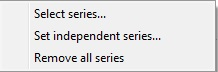
\includegraphics[width=12cm]{images/CSVContextMenu}
\end{center}

The Select Series\ldots option will open a menu to allow you to choose which of
the available series to plot.

\begin{center}
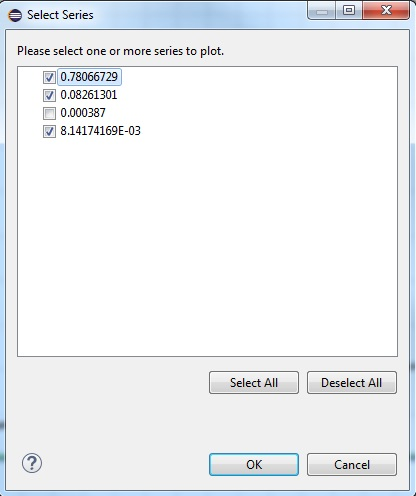
\includegraphics[width=12cm]{images/CSVSelectSeriesDialog}
\end{center}

The Set Independent Series\ldots option will open a menu to allow you to choose
which of the available series to use as the independent series, which will be
used to set the x-axis for the graph.

\begin{center}
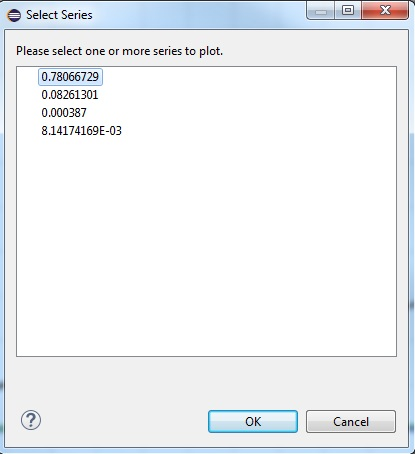
\includegraphics[width=12cm]{images/CSVSelectIndependentSeriesDatabase}
\end{center}

The Remove All Series\ldots option will remove all the graphed series.

\subsection{Interacting with VisIt Plots}

A VisIt plot will contain a 3D visualization of some model. You can click and
drag within the plot to rotate the image and zoom by scrolling your mouse wheel.
Right clicking within the plot will open a context menu. 

\begin{center}
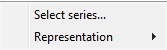
\includegraphics[width=12cm]{images/VisItContextMenu}
\end{center}

Within the Representation submenu will be a list of alternate ways to display
the model. 

At the bottom of the plot will be a series of controls. If your plot does not
have time series data, it will be greyed out. 

\begin{center}

\includegraphics[width=12cm]{images/TimeSliderWidget} 
\end{center}

The yellow arrows will advance/rewind the animation by a single time step. The
play and pasue buttons will begin/halt the animation. The plot can be set to
display an arbitrary time step by either dragging the slider or by typing a time
into the box to its left.

The button on the right will open an options menu to control various other
aspects of the animation.

\begin{center}
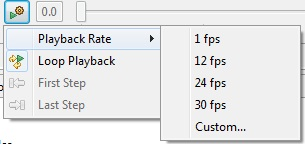
\includegraphics[width=12cm]{images/TimeSliderOptions}
\end{center}

\subsection{Visualizing with 3D graphics}

ICE also contains capabilities to render graphics with the Geometry Editor and
Mesh Editor. Programatically populating these editors with custom input is
beyond the scope of this tutorial. However, what follows will be a brief
overview of the editors' functionality.

\subsubsection{The Geometry Editor}

From the ICE View, the Geometry Editor can be opened with the New Item button,
highlighted below. 

\begin{center}
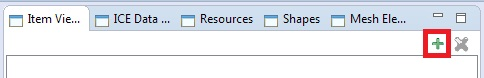
\includegraphics[width=12cm]{images/NewItem}
\end{center}

Select Geometry Editor from the dialog that opens.

\begin{center}
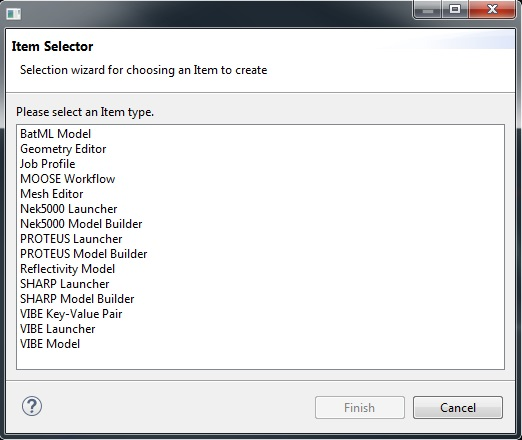
\includegraphics[width=12cm]{images/NewItemDialog}
\end{center}

Clicking the Add Primitives button will display a drop down of primitive shapes
which can be added to the scene.

\begin{center}
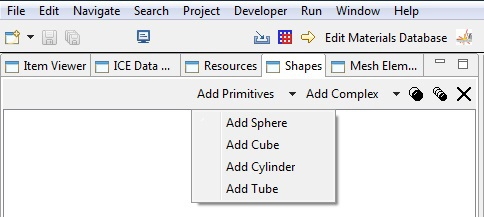
\includegraphics[width=12cm]{images/AddPrimitiveShape}
\end{center}

Complex shapes can similiarly be added using the Add Complex button.

\begin{center}
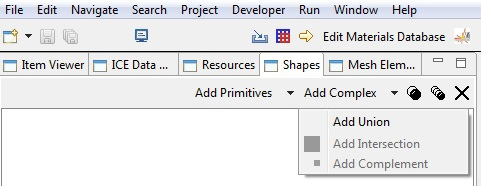
\includegraphics[width=12cm]{images/AddComplexShape}
\end{center}

Primitive shapes can be added under complex shapes by selecting anything beneath
the desired parent complex shape before adding the new primitive.

\begin{center}
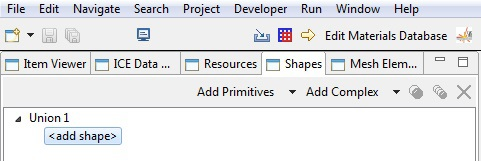
\includegraphics[width=12cm]{images/ComplexShapeTree}
\end{center}

The duplicate button will create an exact copy of the selected shape.

\begin{center}
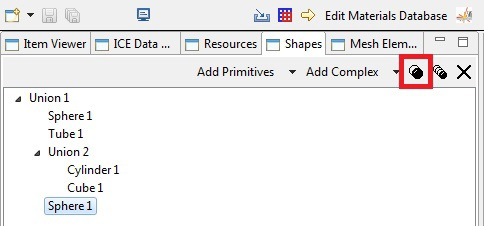
\includegraphics[width=12cm]{images/DuplicateButton}
\end{center}

The replicate button will create many copies with an offest between them.

\begin{center}
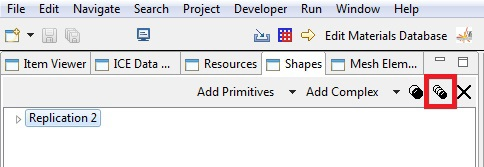
\includegraphics[width=12cm]{images/ReplicateButton}
\end{center}

Pressing it will open a dialog.

\begin{center}
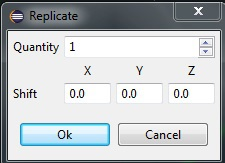
\includegraphics[width=12cm]{images/ReplicateDialog}
\end{center}

The quantity is the number of copies of the shape which should exist, including
the original. The shift is the displacement which will seperate between one
copy and the next

\begin{center}
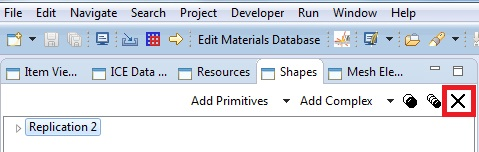
\includegraphics[width=12cm]{images/DeleteButton}
\end{center}

The delete button will delete the selected shape.

\subsubsection{The Mesh Editor}

The Mesh Editor is opened with the Mesh Editor button in the toolbar.

\begin{center}
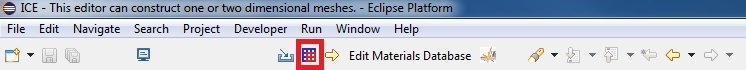
\includegraphics[width=12cm]{images/MeshEditorButton}
\end{center}

Clicking within the grid will create a vertex, until the fourth completes the
polygon.

\begin{center}
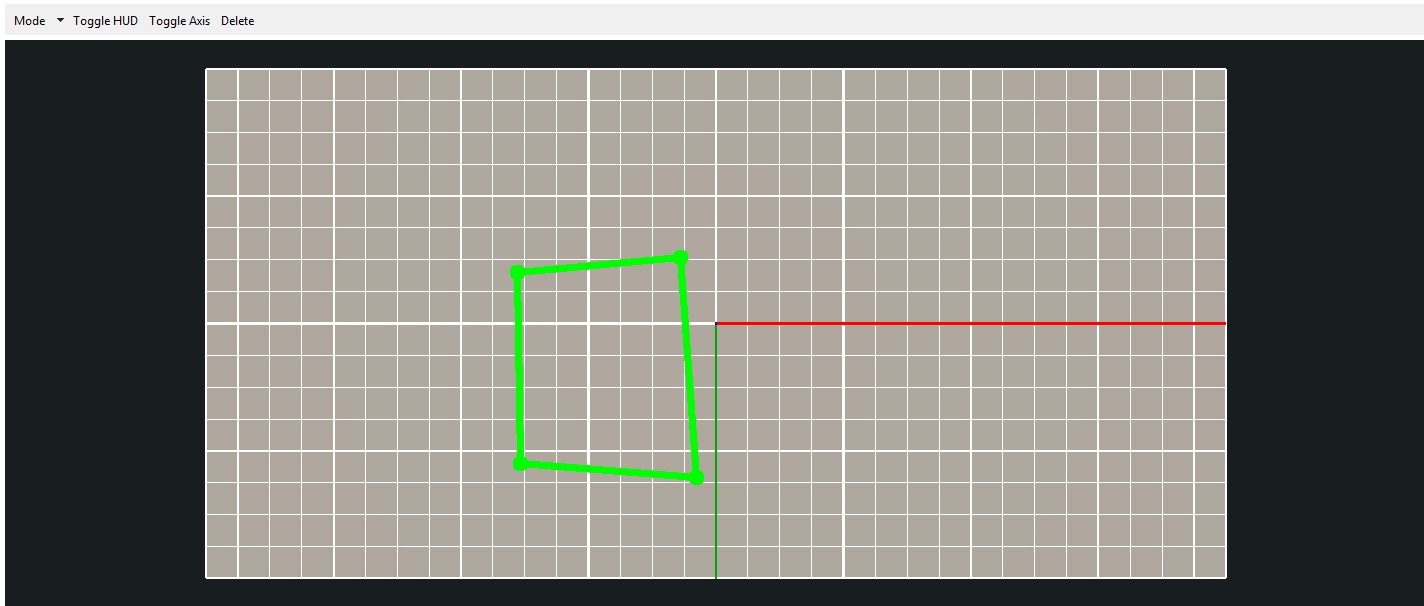
\includegraphics[width=12cm]{images/AddPolygon}
\end{center}

Click again to make the polygon permanent, or hit Esc to cancel.

\begin{center}
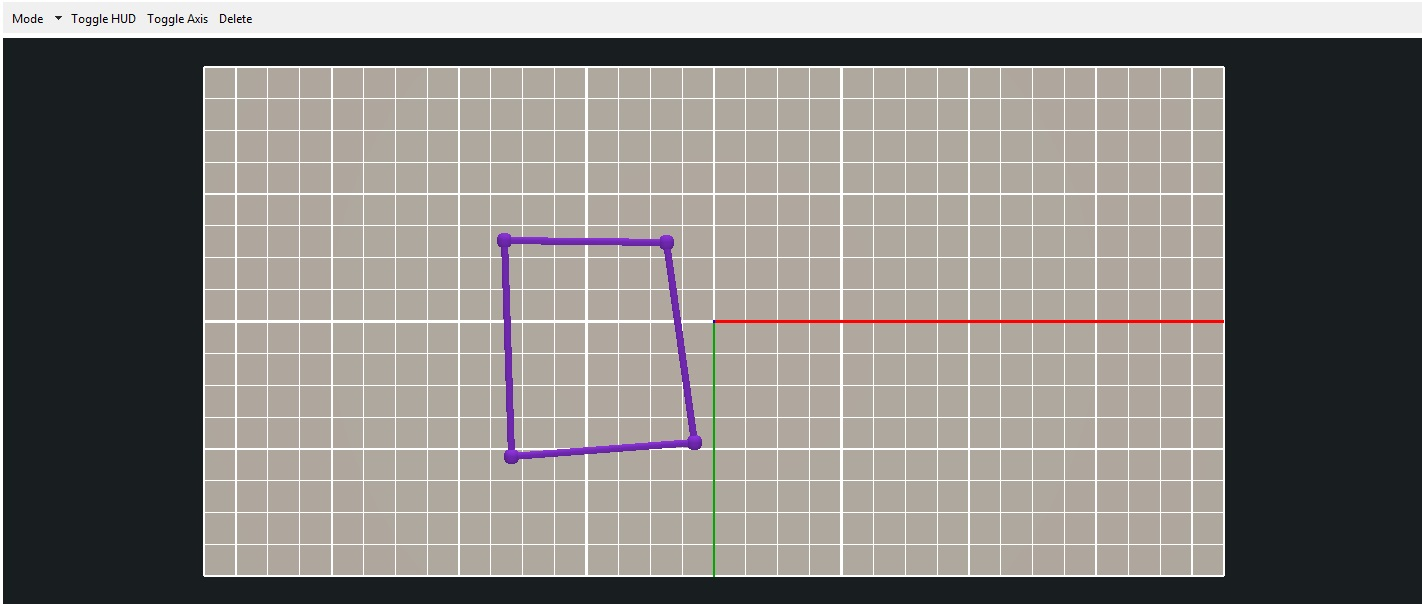
\includegraphics[width=12cm]{images/NewPolygon}
\end{center}

The Mode button in the top left allows you to switch from Add Mode, used
previously, to Edit Mode.

\begin{center}
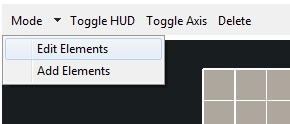
\includegraphics[width=12cm]{images/EditMode}
\end{center}

In Edit Mode, you can click a vertex (or vertices) to select them. 

\begin{center}
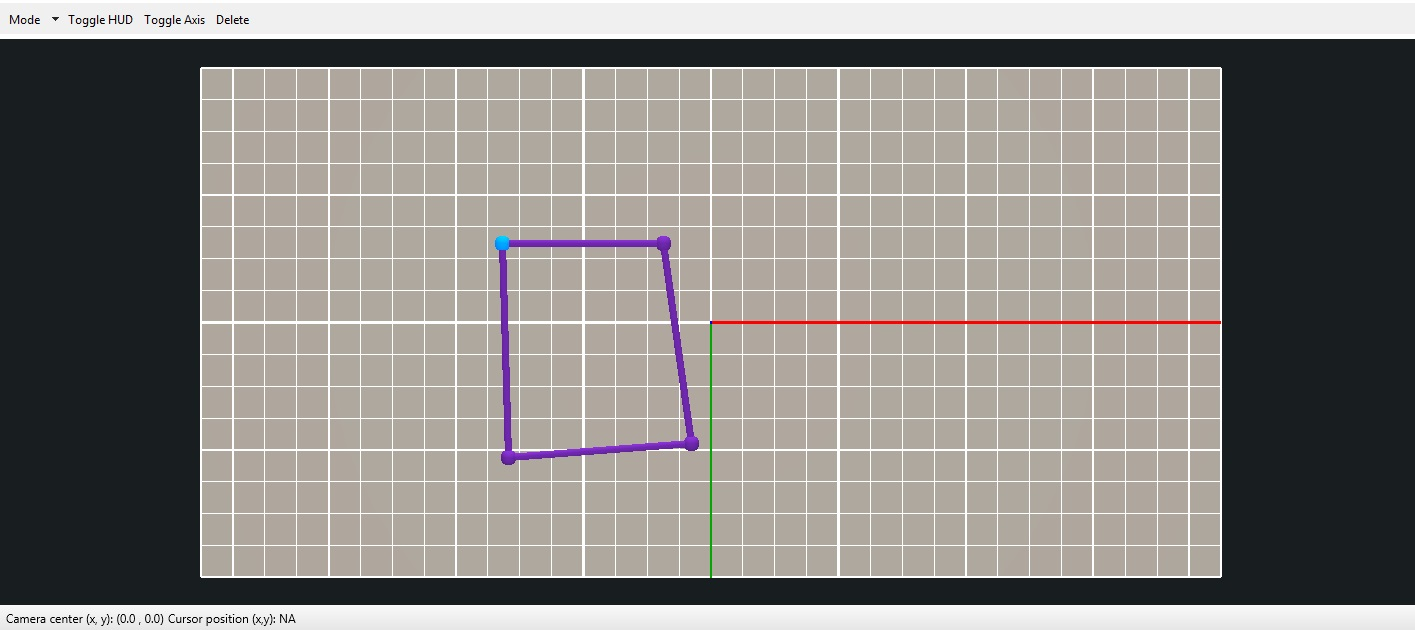
\includegraphics[width=12cm]{images/SelectedVertex}
\end{center}

You can click and drag a vertex to move all selected vertices around the grid.

\begin{center}
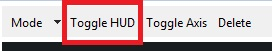
\includegraphics[width=12cm]{images/ToggleHUD}
\end{center}

The Toggle HUD button will toggle the line at the bottom which displays the
camera and cursor positions. 

\begin{center}
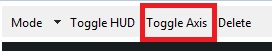
\includegraphics[width=12cm]{images/ToggleAxis}
\end{center}

The Toggle Axis button will show/hide the axes.

\begin{center}
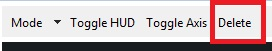
\includegraphics[width=12cm]{images/DeleteMesh}
\end{center}

The Delete button will delete any polygon whose vertices are all selected.

\end{document}
